
% !TeX spellcheck = en_GB
\documentclass{beamer}
\usepackage[utf8]{inputenc}
 \usetheme{antibes}
 \usepackage{movie15}
 \usepackage{graphicx}
 \usepackage{hyperref}
 \usepackage{tikz}
 \usetikzlibrary{shapes.geometric, arrows}
 \tikzstyle{startstop} = [rectangle, rounded corners, minimum width=3cm, minimum height=1cm,text centered, draw=blue, fill=blue!15]
 \tikzstyle{arrow} = [thick,->,>=stealth]
 \hypersetup{
 	colorlinks=true,
 	linkcolor=blue,
 	filecolor=magenta,      
 	urlcolor=cyan,
 }
 
 \urlstyle{same}
 \title[\textcolor{orange}{}] %optional
 {Application of Hilbert-Huang Transform to Bearing Fault Detection}
 
 \subtitle{} 
 \author[] % (optional, for multiple authors)
 {Yapi Donatien Achou}
 
% \institute[VFU] % (optional)
% {
% 	\inst{1}%
% 	Faculty of Physics\\
% 	Very Famous University
% 	\and
% 	\inst{2}%
% 	Faculty of Chemistry\\
% 	Very Famous University
% }
 
 %\date[VLC 2013] % (optional)
 %{Very Large Conference, April 2013}
 
 \logo{
\includegraphics[height=1.5cm]{uib}}
 
 
\begin{document}
 
\frame{\titlepage}
 
 
 %%%%%%%%%%%%%%%%%%%%%%%%%%%%%%%%%%%%%%%%%%%%%%%%%%%%%%%%%%%
 
 
 
 %%%%%%%%%%%%%%%%%%%%%%%%%%%%%%%%%%%%%%%%%%%%%%%%%%%%%%%%%%%%
 
\begin{frame}
\frametitle{Bearings facilitate rotation movements}
\begin{figure}[H]
	\centering
	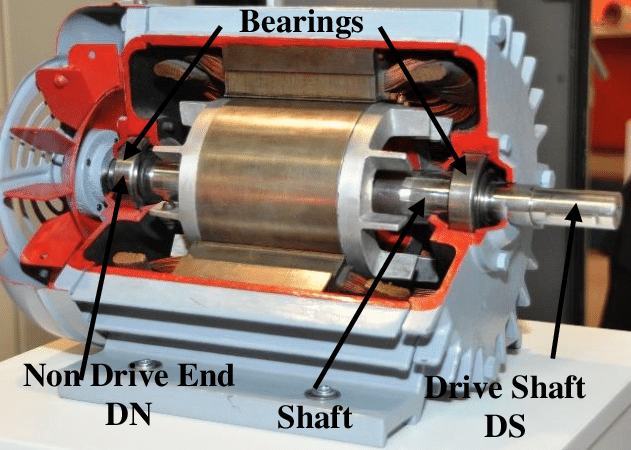
\includegraphics[width=0.8\linewidth]{motor}
	%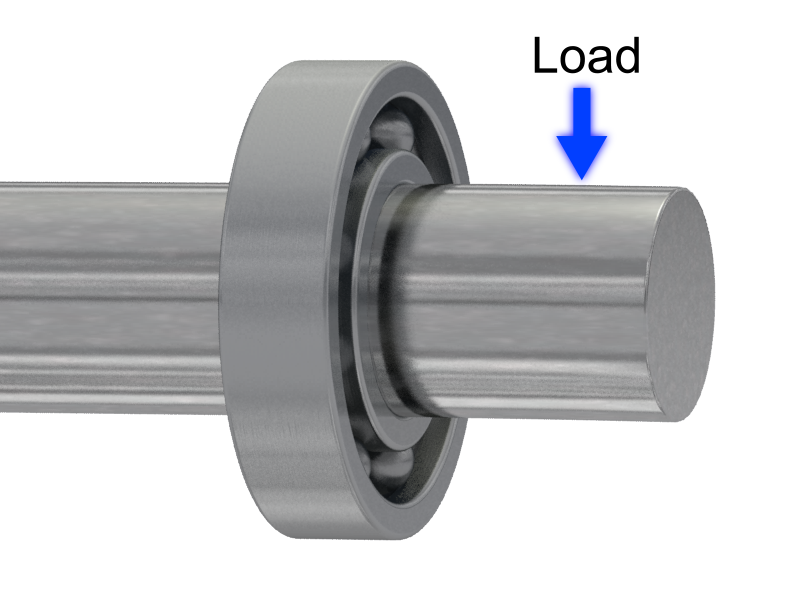
\includegraphics[width=0.4\linewidth]{bearing}
	%\caption{}
	%\label{fig:datascience}
\end{figure}
\end{frame}
%%%%%%%%%%%%%%%%%%%%%%%%%%%%%%%%%%%%%%%%%%%%%%%%%%%%%%
\begin{frame}
	\frametitle{A bearing has multiple components}
	\begin{figure}[H]
		\centering
		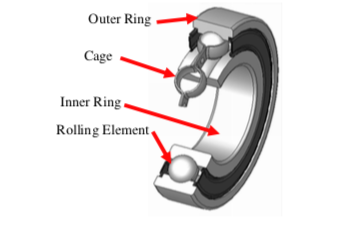
\includegraphics[width=0.5\linewidth]{bearing-geometry1}
		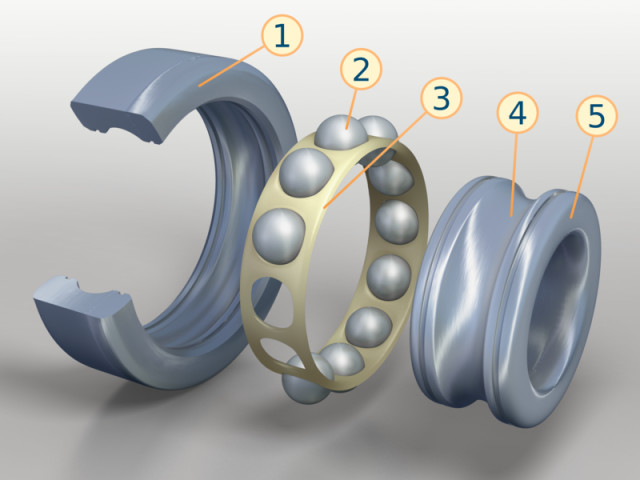
\includegraphics[width=0.5\linewidth]{bearing-geometry2}
		%\caption{}
		%\label{fig:datascience}
	\end{figure}
\end{frame}

%%%%%%%%%%%%%%%%%%%%%%%%%%%%%%%%%%%%%%%%%%%%%%%%%%%%%%

%\begin{frame}
%	\frametitle{Introduction to bearings}
%	\begin{figure}[H]
%		\centering
%		%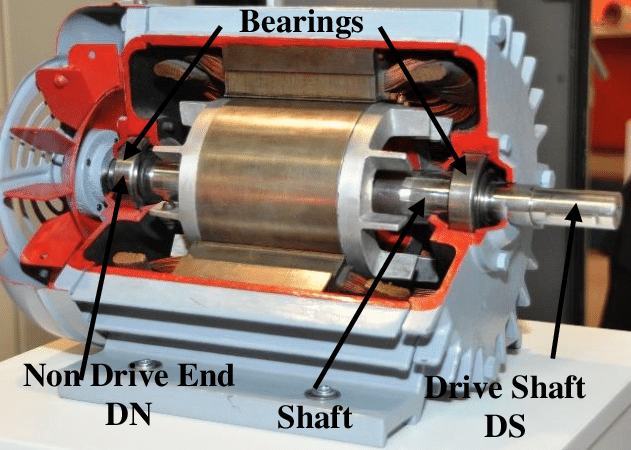
\includegraphics[width=0.8\linewidth]{motor}
%		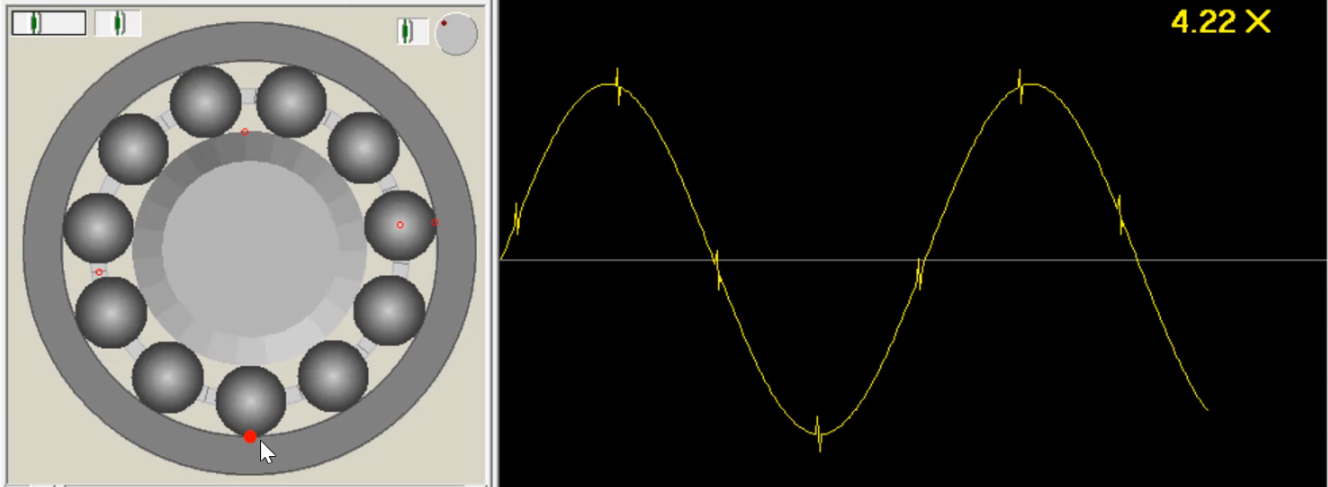
\includegraphics[width=0.8\linewidth]{outer-race1}
%		%\caption{}
%		%\label{fig:datascience}
%	\end{figure}
%\end{frame}

%%%%%%%%%%%%%%%%%%%%%%%%%%%%%%%%%%%%%%%%%%%%%%%%%%%%%%

\begin{frame}
	\frametitle{Bearings are subjected to large forces}
	\begin{figure}[H]
		\centering
		%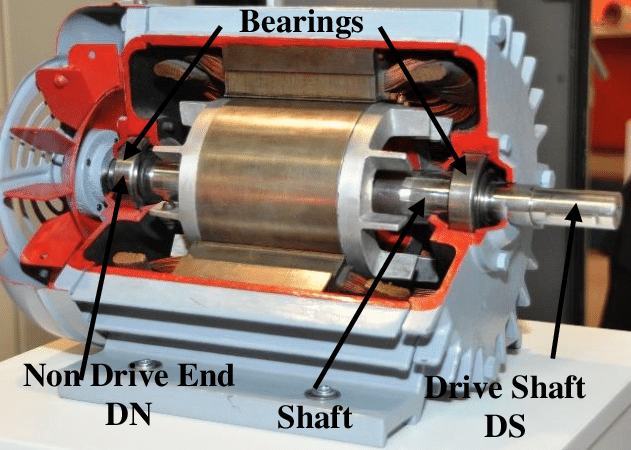
\includegraphics[width=0.8\linewidth]{motor}
		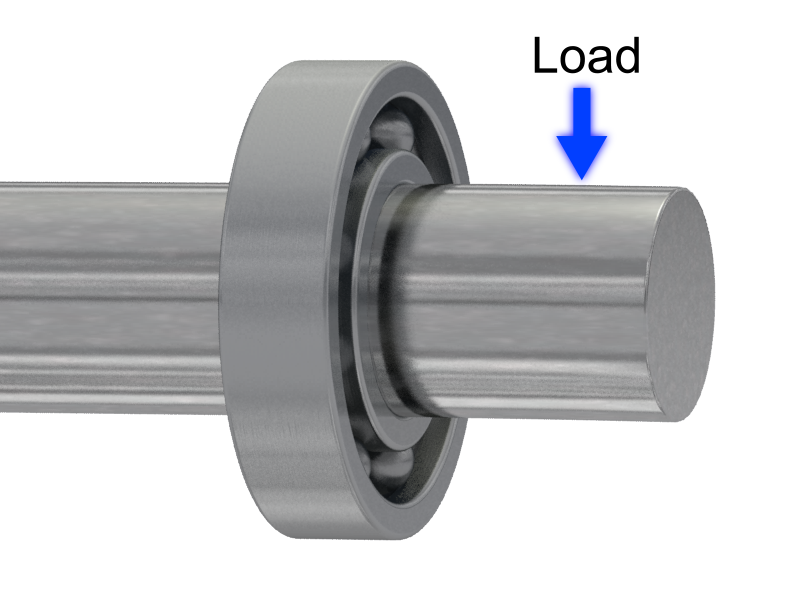
\includegraphics[width=0.8\linewidth]{bearing}
		%\caption{}
		%\label{fig:datascience}
	\end{figure}
\end{frame}

%%%%%%%%%%%%%%%%%%%%%%%%%%%%%%%%%%%%%%%%%%%%%%%%%%%%%%%%

\begin{frame}
	\frametitle{Fault can result as a consequences of load}
	\begin{figure}[H]
		\centering
		%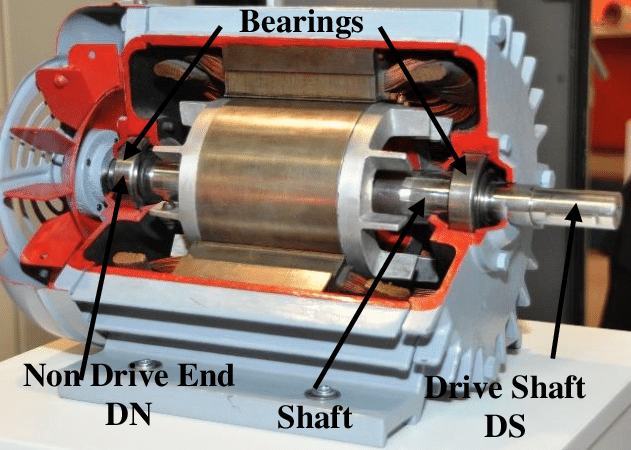
\includegraphics[width=0.8\linewidth]{motor}
		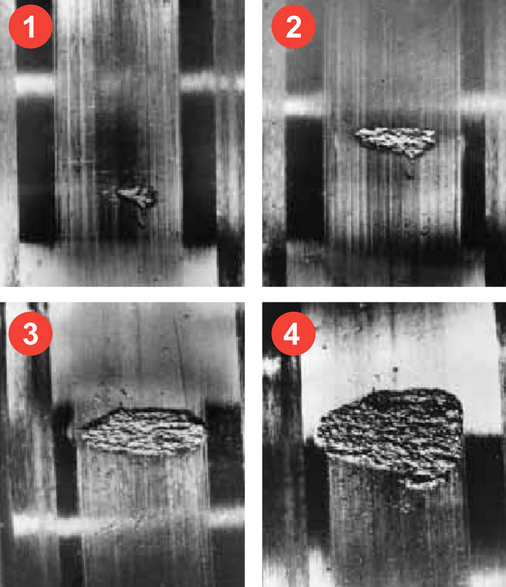
\includegraphics[width=0.6\linewidth]{bearing_fault_evolution}
		%\caption{}
		%\label{fig:datascience}
	\end{figure}
\end{frame}
%%%%%%%%%%%%%%%%%%%%%%%%%%%%%%%%%%%%%%%%%%%%%%%%%%%%%%%%


\begin{frame}
	\frametitle{Bearing faults generate high frequency shock}
	\begin{figure}[H]
		\centering
		%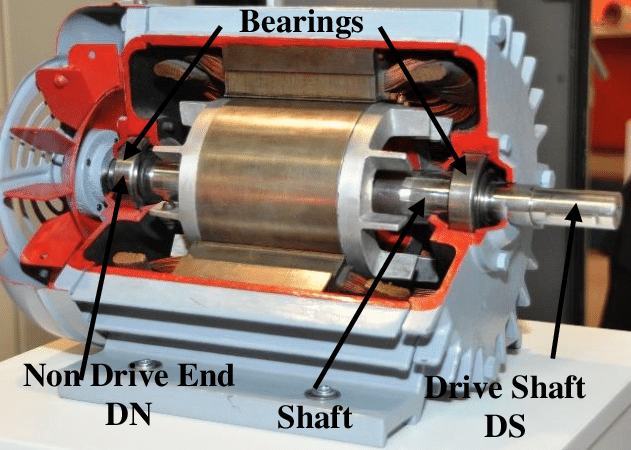
\includegraphics[width=0.8\linewidth]{motor}
		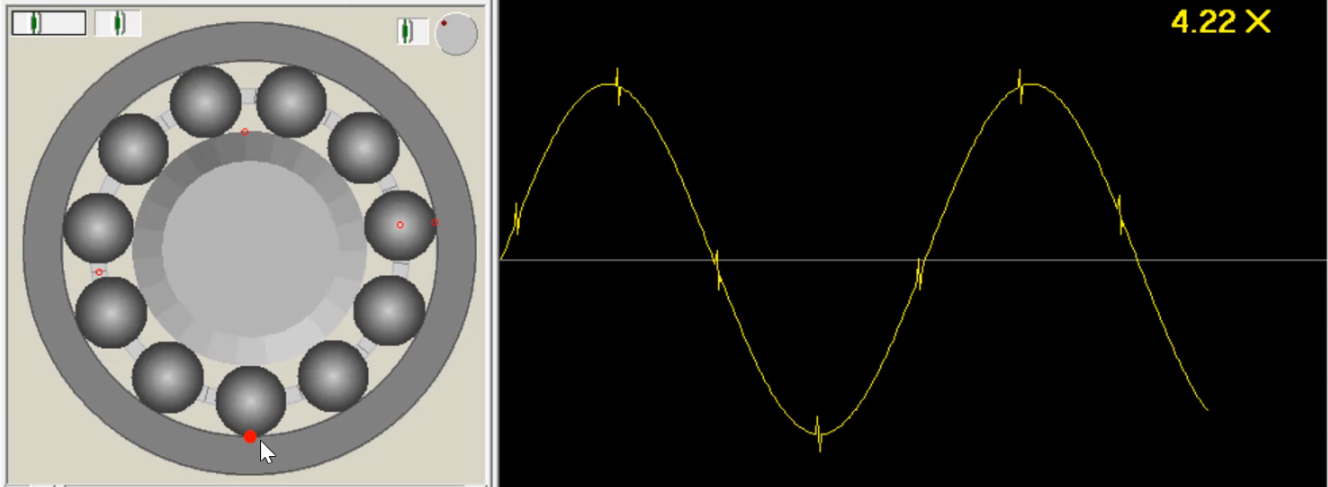
\includegraphics[width=0.8\linewidth]{outer-race1}
		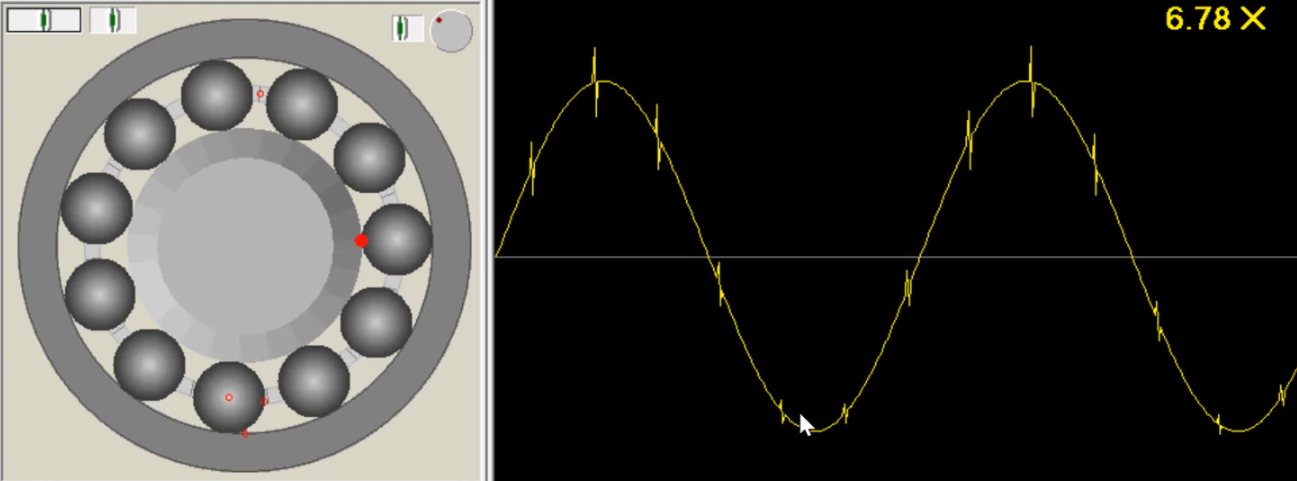
\includegraphics[width=0.8\linewidth]{inner-race1}
		%\caption{}
		%\label{fig:datascience}
	\end{figure}
\end{frame}

%%%%%%%%%%%%%%%%%%%%%%%%%%%%%%%%%%%%%%%%%%%%%%%%%%%%%%%%
\begin{frame}
	\frametitle{Bearings inner race and outer race shock are different}
	\begin{figure}[H]
		\centering
		%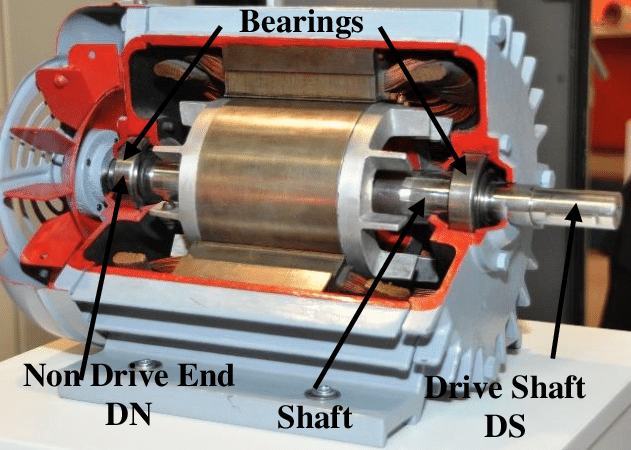
\includegraphics[width=0.8\linewidth]{motor}
		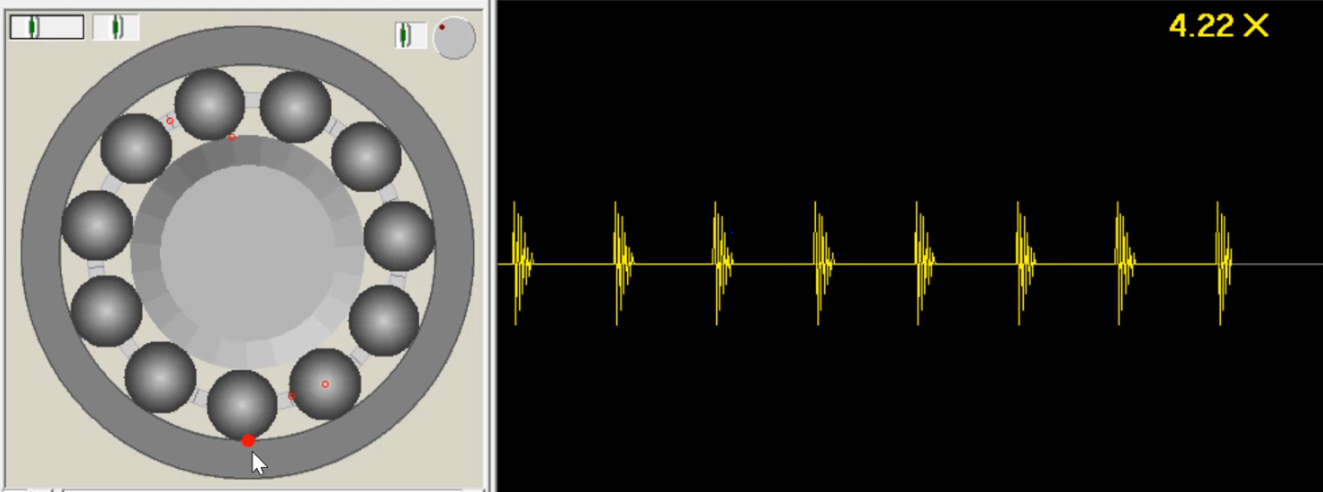
\includegraphics[width=0.8\linewidth]{outer-race2}
		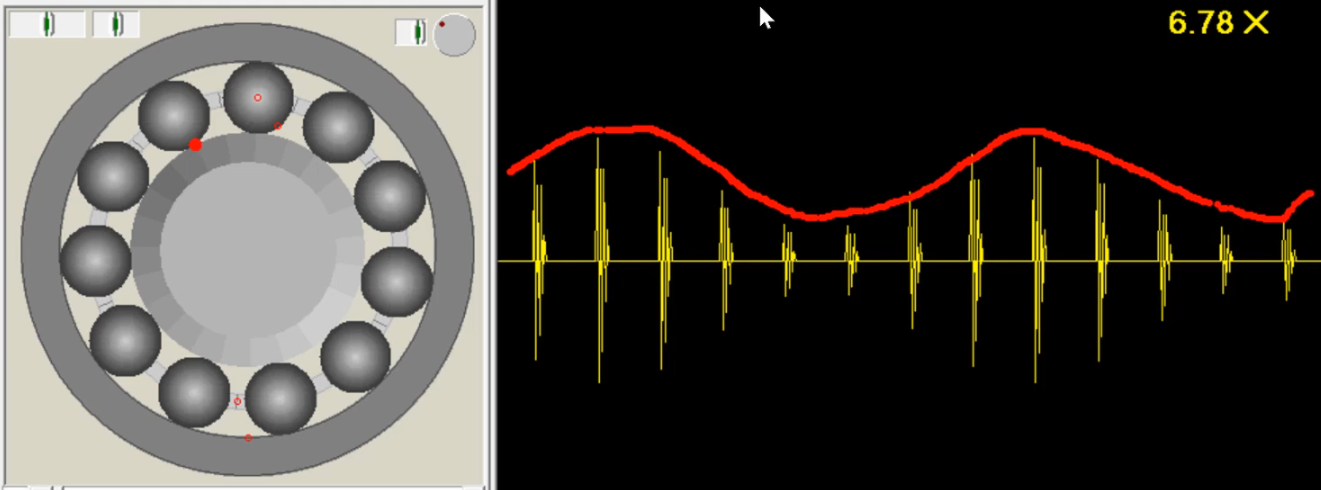
\includegraphics[width=0.8\linewidth]{inner-race2}
		%\caption{}
		%\label{fig:datascience}
	\end{figure}
\end{frame}

%%%%%%%%%%%%%%%%%%%%%%%%%%%%%%%%%%%%%%%%%%%%%%%%%%%%%%%%%



%%%%%%%%%%%%%%%%%%%%%%%%%%%%%%%%%%%%%%%%%%%%%%%%%%%%%%%%
\begin{frame}
	\frametitle{The High frequency Resonance Technique isolates bearing fault vibration}
	\begin{figure}[H]
		\centering
		%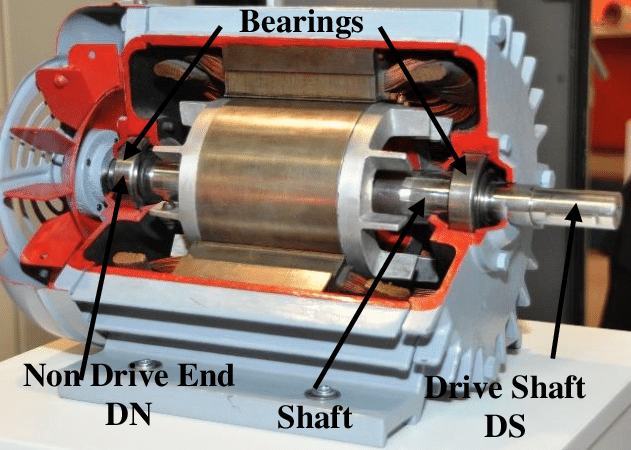
\includegraphics[width=0.8\linewidth]{motor}
		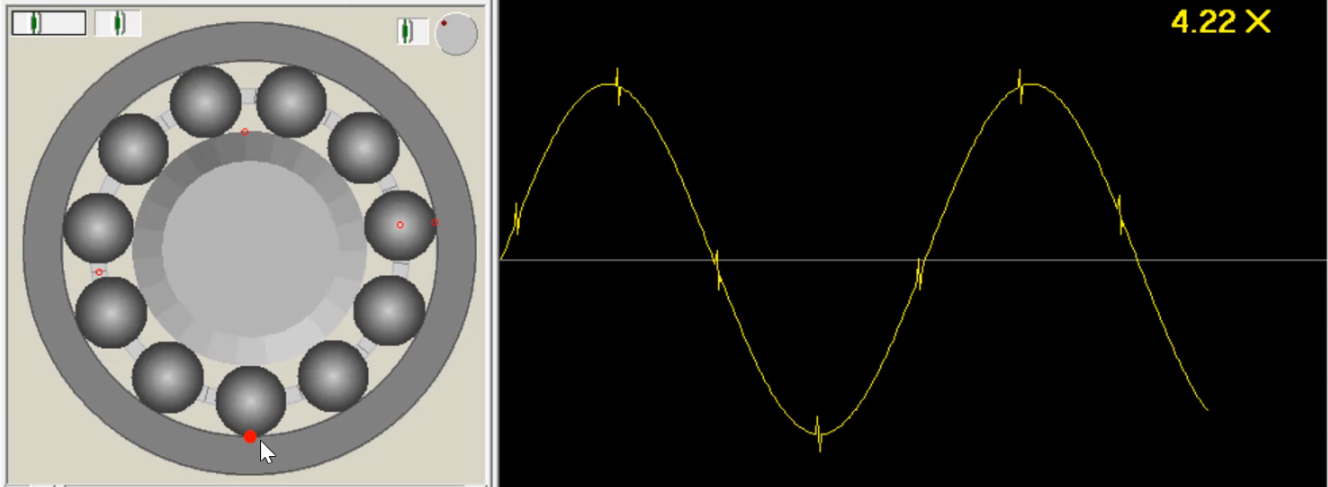
\includegraphics[width=0.8\linewidth]{outer-race1}
		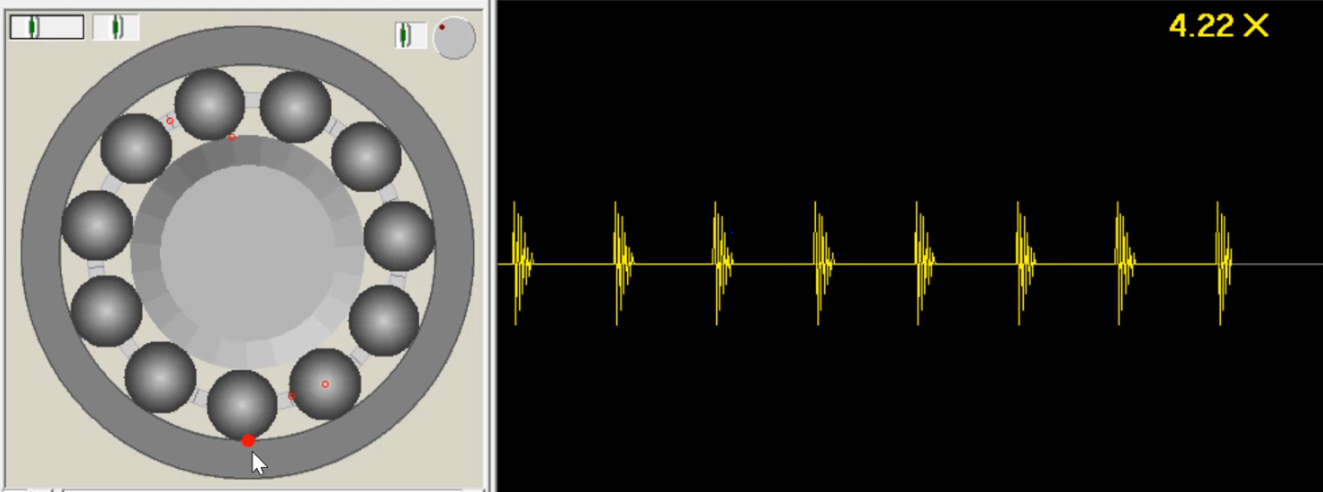
\includegraphics[width=0.8\linewidth]{outer-race2}
		%\caption{}
		%\label{fig:datascience}
	\end{figure}
\end{frame}

%%%%%%%%%%%%%%%%%%%%%%%%%%%%%%%%%%%%%%%%%%%%%%%%%%%%%%%%%

%%%%%%%%%%%%%%%%%%%%%%%%%%%%%%%%%%%%%%%%%%%%%%%%%%%%%%%%
\begin{frame}
	\frametitle{The High frequency Resonance Technique filters a target vibration signal}
	\begin{figure}[H]
		\centering
		%signal, butter_band_pass, envelop
		%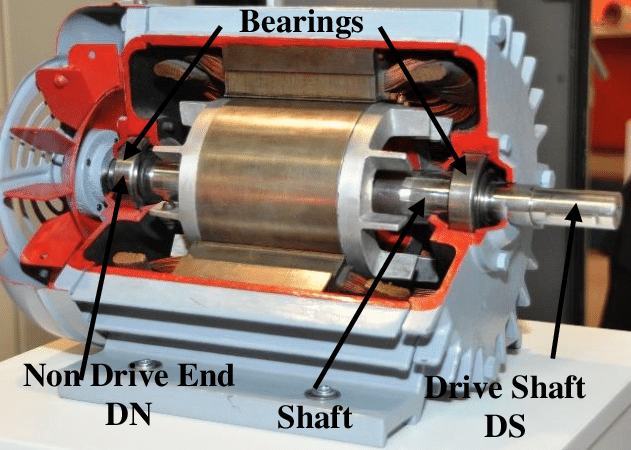
\includegraphics[width=0.8\linewidth]{motor}
		%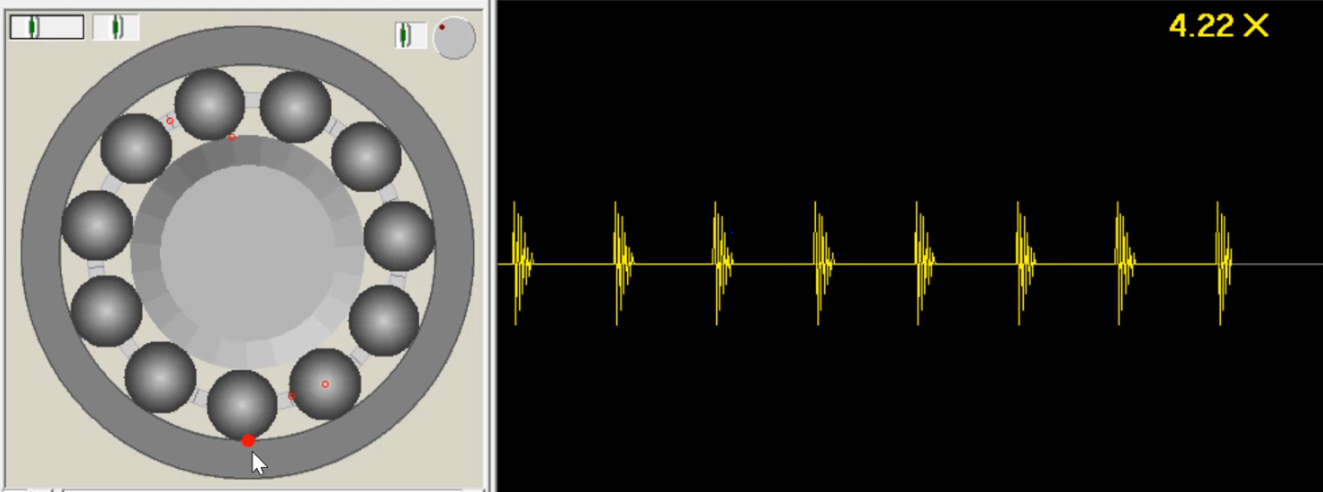
\includegraphics[width=0.8\linewidth]{outer-race2}
		%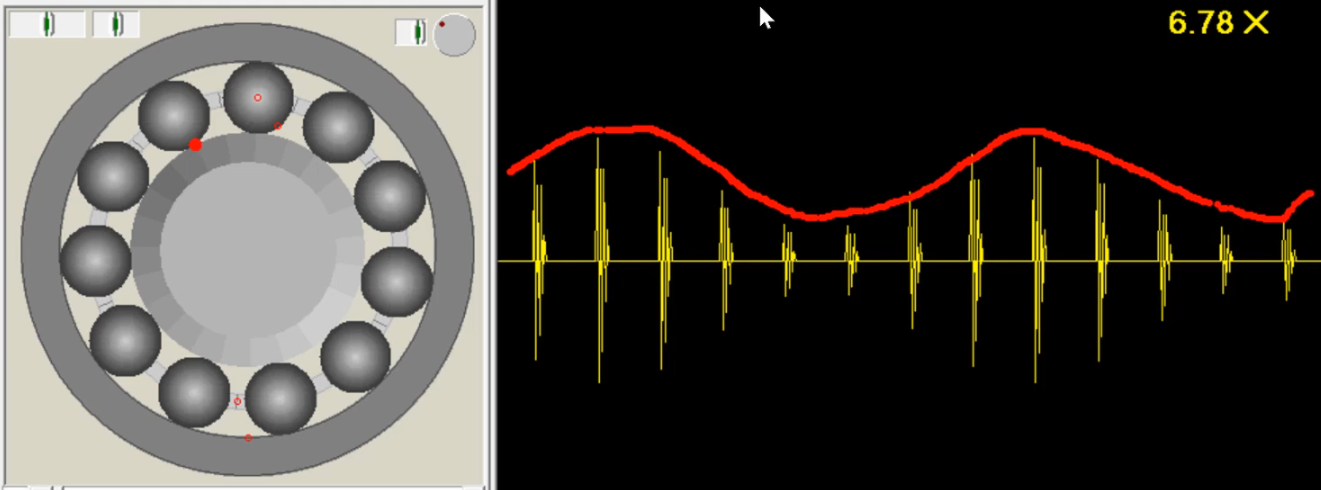
\includegraphics[width=0.8\linewidth]{inner-race2}
		%\caption{}
		%\label{fig:datascience}
	\end{figure}
\end{frame}

%%%%%%%%%%%%%%%%%%%%%%%%%%%%%%%%%%%%%%%%%%%%%%%%%%%%%%%%%


%%%%%%%%%%%%%%%%%%%%%%%%%%%%%%%%%%%%%%%%%%%%%%%%%%%%%%%%
\begin{frame}
	\frametitle{A bearing fault is revealed through the Fourier transform}
	\begin{figure}[H]
		\centering
		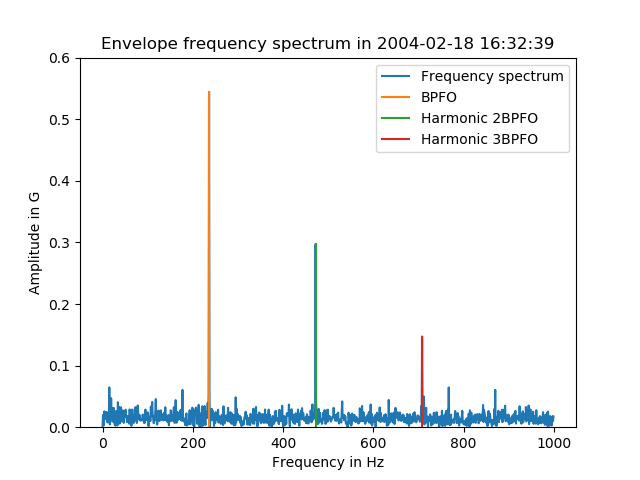
\includegraphics[width=0.45\linewidth]{last_day_spectrum_bpfo}
		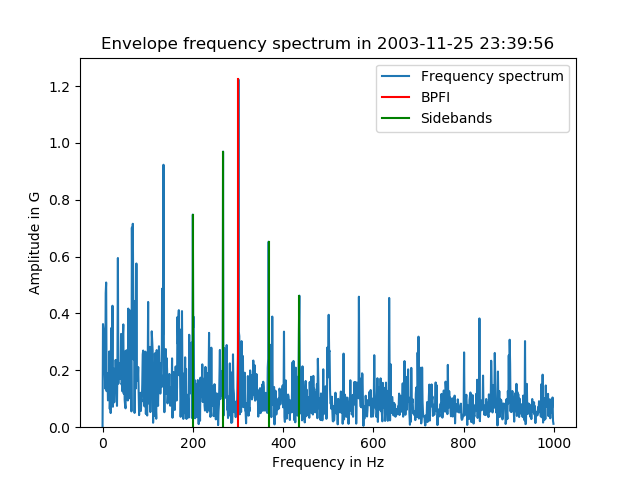
\includegraphics[width=0.45\linewidth]{bpfi_sidebands}
		%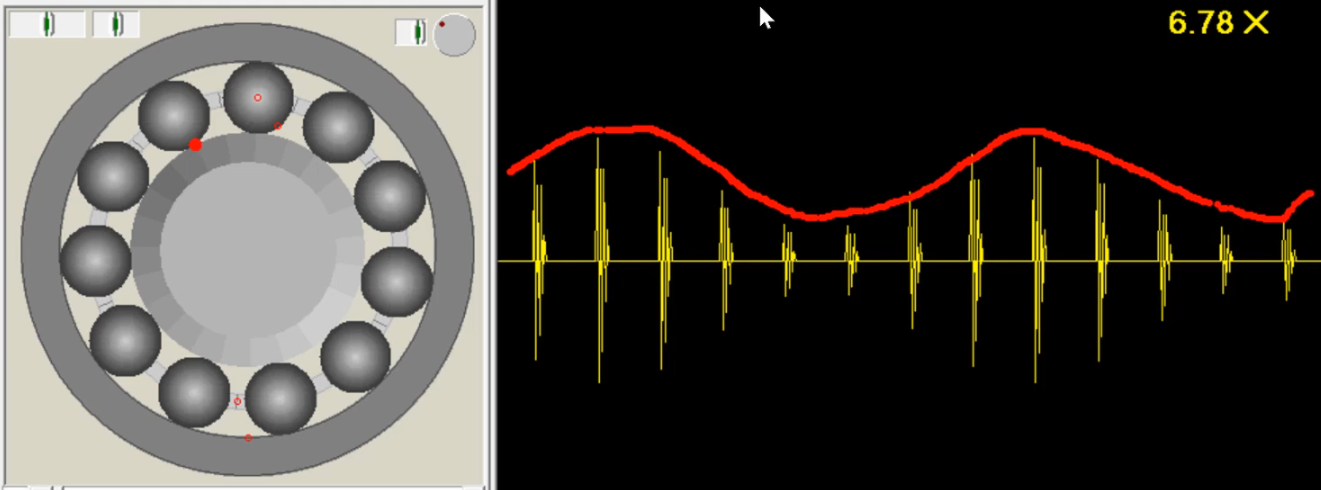
\includegraphics[width=0.8\linewidth]{inner-race2}
		%\caption{}
		%\label{fig:datascience}
	\end{figure}
\end{frame}

%%%%%%%%%%%%%%%%%%%%%%%%%%%%%%%%%%%%%%%%%%%%%%%%%%%%%%%%%
\end{document}

